\documentclass[xetex,mathserif,serif]{beamer}
\usepackage{polyglossia}
\setdefaultlanguage[babelshorthands=true]{russian}
\usepackage{minted}
\usepackage{tabu}
\usepackage{moresize}

\useoutertheme{infolines}

\usepackage{fontspec}
\setmainfont{FreeSans}
\newfontfamily{\russianfonttt}{FreeSans}

\definecolor{links}{HTML}{2A1B81}
\hypersetup{colorlinks,linkcolor=,urlcolor=links}

\setbeamertemplate{blocks}[rounded][shadow=false]

\setbeamercolor*{block title alerted}{fg=red!50!black,bg=red!20}
\setbeamercolor*{block body alerted}{fg=black,bg=red!10}

\tabulinesep=1.2mm

\title{.NET Internals}
\author[Юрий Литвинов]{Юрий Литвинов\\\small{\textcolor{gray}{y.litvinov@spbu.ru}}}
\date{30.11.2018г}

\newcommand{\attribution}[1] {
\vspace{-5mm}\begin{flushright}\begin{scriptsize}\textcolor{gray}{\textcopyright\, #1}\end{scriptsize}\end{flushright}
}

\begin{document}

	\frame{\titlepage}

	\section{Введение}

	\begin{frame}
		\frametitle{Работа с ресурсами}
		\begin{itemize}
			\item Выделить память под объект, представляющий ресурс
			\item Инициализировать ресурс
			\item Использовать ресурс, вызывая методы объекта
			\item Деинициализировать ресурс
			\item Освободить память
		\end{itemize}
		В отличие от C++, .NET не даст испортить память (без \textbf{unsafe}) и уменьшает вероятность утечек памяти
	\end{frame}

	\begin{frame}
		\frametitle{Выделение ресурсов}
		\framesubtitle{Managed Heap}
		\begin{itemize}
			\item Вычисление размера объекта
			\begin{itemize}
				\item Поля объекта + поля, унаследованные от предка
			\end{itemize}
			\item Добавление служебных данных
			\begin{itemize}
				\item Указатель на объект-тип
				\item Sync block index
			\end{itemize}
			\item Проверка наличия свободного места на куче
			\item Сброс памяти в 0, вызов конструктора, возврат указателя на объект из \textbf{new}
			\begin{itemize}
				\item Прямо перед возвратом продвигается указатель начала свободного места в куче
			\end{itemize}
		\end{itemize}
		\begin{center}
			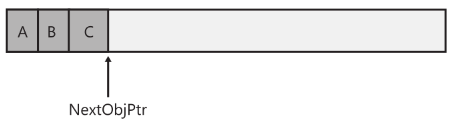
\includegraphics[width=0.4\textwidth]{heapAllocation.png}
		\end{center}
	\end{frame}

	\begin{frame}
		\frametitle{Особенности}
		\begin{itemize}
			\item Managed Heap выделяется при запуске процесса, но может расти
			\begin{itemize}
				\item Доступно порядка 1.5Гб для 32-битных систем и порядка 8Тб для 64-битных
			\end{itemize}
			\item Выделение памяти --- просто прибавить размер объекта к указателю
			\begin{itemize}
				\item Делается мгновенно, в отличие от C++
			\end{itemize}
			\item Объекты лежат друг за другом подряд
			\begin{itemize}
				\item Занимают возможно мало страниц памяти
				\item С большей вероятностью помещаются в кеш процессора
			\end{itemize}
		\end{itemize}
	\end{frame}

	\section{Сборка мусора}

	\begin{frame}
		\frametitle{Сборка мусора, mark}
		\begin{itemize}
			\item \textbf{roots} --- переменные ссылочных типов, лежащие на стеке
			\item \textbf{marking} --- пометка всех объектов, достижимых из roots, как живых
			\begin{itemize}
				\item Исполнение всех потоков прерывается
				\item Все объекты помечаются как мёртвые
				\begin{itemize}
					\item Бит в sync block index
				\end{itemize}
				\item Гонится обход графа от root-ов
			\end{itemize}
		\end{itemize}
		\begin{center}
			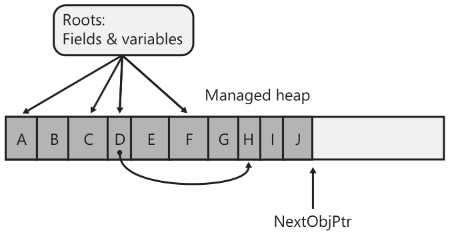
\includegraphics[width=0.4\textwidth]{heapBeforeCollection.png}
		\end{center}
	\end{frame}

	\begin{frame}
		\frametitle{Сборка мусора, sweep}
		\begin{itemize}
			\item ``Сжатие кучи'' --- все живые объекты сдвигаются в куче так, чтобы занимать непрерывный участок памяти
			\begin{itemize}
				\item Восстанавливается locality of reference
				\item Исключается фрагментирование памяти
				\begin{itemize}
					\item Чтобы выделение можно было и дальше осуществлять просто сдвигом указателя
				\end{itemize}
			\end{itemize}
			\item Ссылки в живых объектах редактируются с учётом сдвигов
			\item Потоки продолжают выполнение
			\item Если после сборки мусора памяти всё ещё не хватает, из new бросается OutOfMemoryException
			\item Статические поля живут вечно  % Хороший способ прострелить себе ногу --- сделать статический список и добавлять туда объекты, не удаляя их
		\end{itemize}
		\begin{center}
			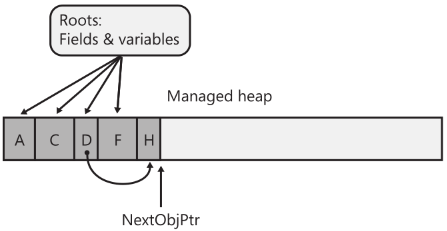
\includegraphics[width=0.4\textwidth]{heapAfterCollection.png}
		\end{center}
	\end{frame}

	\begin{frame}[fragile]
		\frametitle{Пример}
		\begin{footnotesize}
			\begin{minted}{csharp}
public static class Program {
    public static void Main() {
        // Create a Timer object that knows to call our TimerCallback
        // method once every 2000 milliseconds.
        Timer t = new Timer(TimerCallback, null, 0, 2000);
        // Wait for the user to hit <Enter>
        Console.ReadLine();
    }

    private static void TimerCallback(Object o) {
        // Display the date/time when this method got called.
        Console.WriteLine("In TimerCallback: " + DateTime.Now);
        // Force a garbage collection to occur for this demo.
        GC.Collect();
    }
}
			\end{minted}
			% При сборке под релизом и запуске оказывается, что колбэк вызывается 1 раз --- поскольку t не используется ниже в теле метода, компилятор не считает её рутом и убивает таймер.
			% А вот если собрать всё под дебагом, то всё будет работать ожидаемо --- дебаггер не знает, не захочет ли пользователь просмотреть значение t ниже по коду, поэтому JIT искусственно продлевает 
			% жизнь таймера до выхода t из области видимости.
			% С ключом /optimize+ таже под дебагом оно будет работать как под релизом.
		\end{footnotesize}
	\end{frame}

	\begin{frame}[fragile]
		\frametitle{Так тоже будет плохо}
		\begin{footnotesize}
			\begin{minted}{csharp}
public static class Program {
    public static void Main() {
        // Create a Timer object that knows to call our TimerCallback
        // method once every 2000 milliseconds.
        Timer t = new Timer(TimerCallback, null, 0, 2000);
        // Wait for the user to hit <Enter>
        Console.ReadLine();
        // Refer to t after ReadLine (this gets optimized away)
        t = null;
    }

    private static void TimerCallback(Object o) {
        // Display the date/time when this method got called.
        Console.WriteLine("In TimerCallback: " + DateTime.Now);
        // Force a garbage collection to occur for this demo.
        GC.Collect();
    }
}
			\end{minted}
		\end{footnotesize}
	\end{frame}

	\begin{frame}[fragile]
		\frametitle{А вот так будет ок}
		\begin{footnotesize}
			\begin{minted}{csharp}
public static class Program {
    public static void Main() {
        // Create a Timer object that knows to call our TimerCallback
        // method once every 2000 milliseconds.
        Timer t = new Timer(TimerCallback, null, 0, 2000);
        // Wait for the user to hit <Enter>
        Console.ReadLine();
        // Refer to t after ReadLine (t will survive GCs until Dispose returns)
        t.Dispose();
    }

    private static void TimerCallback(Object o) {
        // Display the date/time when this method got called.
        Console.WriteLine("In TimerCallback: " + DateTime.Now);
        // Force a garbage collection to occur for this demo.
        GC.Collect();
    }
}
			\end{minted}
		\end{footnotesize}
		% Тут надо сказать, что таймер --- это чит, потому что это чуть ли не единственный класс в .NET, для которого можно наблюдать эффекты, связанные со сборкой мусора --- само существование таймера на куче заставляет пул потоков дёргать обработчик.
		% Для остальных классов таких побочных эффектов нет, поэтому сборка мусора не произойдёт, пока существование объекта хоть как-то отразится на функционировании программы (конечно, если всё managed, сборщик мусора ничего не знает про native-код).
	\end{frame}

	\section{Сборка мусора}

	\begin{frame}
		\frametitle{Не всё так просто}
		\framesubtitle{Поколения}
		Каждый раз чистить память во всей куче было бы дорого, поэтому придумали поколения:
		\begin{itemize}
			\item Чем новее объект, тем меньше, скорее всего, он будет нужен
			\begin{itemize}
				\item Различного рода локальные переменные и переменные внутри тел циклов
			\end{itemize}
			\item Чем дольше объект живёт, тем дольше, скорее всего, он ещё проживёт
			\item Собирать память в части кучи можно быстрее, чем во всей куче
		\end{itemize}
		Все новые объекты добавляются в поколение 0:
		\begin{center}
			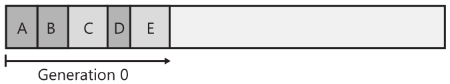
\includegraphics[width=0.4\textwidth]{generation0.png}
		\end{center}
	\end{frame}

	\begin{frame}
		\frametitle{Первая сборка мусора}
		\begin{itemize}
			\item Под поколение 0 выделяется ``бюджет'' памяти
			\item При переполнении поколения 0 происходит сборка мусора и все выжившие объекты перемещаются в поколение 1
			\begin{itemize}
				\item Поколение 0 после GC всегда пусто
			\end{itemize}
		\end{itemize}
		\begin{center}
			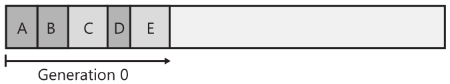
\includegraphics[width=0.4\textwidth]{generation0.png}
		\end{center}
		\begin{itemize}
			\item Следующие выделения идут в поколение 0
			\item Объекты в поколении 1 могут стать недостижимы
		\end{itemize}
		\begin{center}
			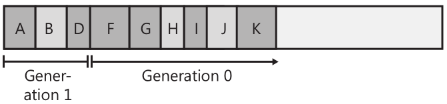
\includegraphics[width=0.4\textwidth]{generation1.png}
		\end{center}
	\end{frame}

	\begin{frame}
		\frametitle{Последующие сборки мусора}
		\begin{footnotesize}
			\begin{itemize}
				\item Сборки мусора в Gen0 игнорируют Gen1, пока бюджет первого поколения не превышен
				\begin{itemize}
					\item \begin{scriptsize}При JIT-е для записи в поле ссылочного типа генерируется Write Barrier\end{scriptsize}
					\item \begin{scriptsize}Write Barrier выставляет флаг в Card Table, если объект в поколении 1 или 2\end{scriptsize}
					\item \begin{scriptsize}Сборщик мусора смотрит на Card Table, не обходя объекты из Gen1 и Gen2\end{scriptsize}
					\item \begin{scriptsize}Если есть изменения, то честно гонится обход и объекты помечаются как живые\end{scriptsize}
					\item \begin{scriptsize}После сборки мусора Card Table сбрасывается\end{scriptsize}
					\item \begin{scriptsize}Несколько медленнее запись в поля ссылочных типов, но значительно быстрее сборка мусора\end{scriptsize}
				\end{itemize}
				\item Недостижимые объекты в Gen1 могут пережить сборку мусора
				\item Сборка мусора в поколении 0 сравнима по времени с page fault (меньше миллисекунды)
			\end{itemize}
		\end{footnotesize}
		\begin{center}
			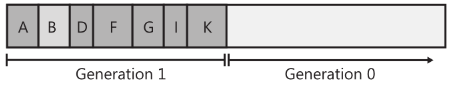
\includegraphics[width=0.4\textwidth]{generation1updated.png}
		\end{center}
	\end{frame}

	\begin{frame}
		\frametitle{Что дальше}
		Если бюджет поколения 1 превышен, запускается сборка мусора и выжившие объекты перемещаются в поколение 2:
		\begin{center}
			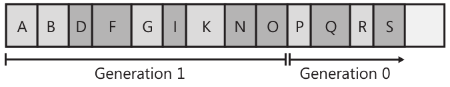
\includegraphics[width=0.4\textwidth]{generation1full.png}
		\end{center}
		
		\vspace{-7mm}
		
		\begin{center}\begin{LARGE}$\downarrow$\end{LARGE}\end{center}
	
		\vspace{-7mm}
	
		\begin{center}
			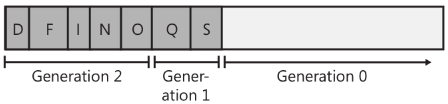
\includegraphics[width=0.4\textwidth]{generation2.png}
		\end{center}
		Больше поколений не бывает (GC.MaxGeneration возвращает 2)

		Сборщик мусора динамически управляет бюджетами на поколения
		\begin{itemize}
			\item Если выживших в поколении мало, бюджет уменьшается
			\item Сборки мусора происходят чаще, но быстрее, и надо меньше памяти
		\end{itemize}
	\end{frame}

	\section{Fine tuning}

	\begin{frame}
		\frametitle{Когда происходит сборка мусора}
		\begin{itemize}
			\item Закончился бюджет на поколение 0
			\item Явный вызов System.GC.Collect
			\begin{itemize}
				\item Настоятельно не рекомендуется
			\end{itemize}
			\item ОС сообщает о нехватке памяти
			\begin{itemize}
				\item Да, CLR подписывается на события ОС
			\end{itemize}
			\item Выгружается AppDomain
			\begin{itemize}
				\item Выполняется финализация всех объектов
			\end{itemize}
			\item Нормально завершается процесс с приложением
			\begin{itemize}
				\item В отличие от убийства процесса через Task Manager
				\item Выполняется только финализация, сжатие кучи не делается
			\end{itemize}
		\end{itemize}
	\end{frame}

	\begin{frame}
		\frametitle{Large Object Heap}
		\begin{itemize}
			\item Объекты размером больше примерно 85000 байт живут по особым правилам
			\item Отдельная куча для таких объектов
			\item Не происходит сжатие кучи
			\begin{itemize}
				\item Возможна фрагментация
				\item Возможен OutOfMemoryException из-за фрагментации
			\end{itemize}
			\item Они всегда считаются в поколении 2
			\begin{itemize}
				\item Короткоживущие большие объекты заставляют GC страдать
			\end{itemize}
		\end{itemize}
	\end{frame}

	\begin{frame}[fragile]
		\frametitle{Режимы сборки мусора}
		\begin{itemize}
			\item Workstation --- частая быстрая сборка на одном ядре, чтобы не тормозить подолгу и не мешать другим приложениям
			\begin{itemize}
				\item По умолчанию
			\end{itemize}
			\item Server --- многопоточная сборка, занимающая весь процессор (считается, что приложение на сервере одно)
			\begin{itemize}
				\item На одноядерной машине бесполезен и не используется
			\end{itemize}
		\end{itemize}
		App.config/Web.config, включающий серверный GC:
		\begin{footnotesize}
			\begin{minted}{xml}
<configuration>
    <runtime>
        <gcServer enabled="true"/>
    </runtime>
</configuration>
			\end{minted}
		\end{footnotesize}
	\end{frame}

	\begin{frame}[fragile]
		\frametitle{Многопоточная сборка}
		\begin{footnotesize}
			\begin{itemize}
				\item Не Server-режим!
				\item Mark выполняется в отдельном потоке во время работы приложения
				\item Если требуется сборка поколений 0 или 1, всё работает как обычно
				\item Если требуется сборка поколения 2, в поколении 0 выделяется объект вне бюджета и приложение продолжает работать
				\item В это время гонится mark по поколению 2 в отдельном потоке
				\item Когда закончили, останавливаем потоки и выполняем sweep
				\item Mark уже пометил большинство достижимых объектов, так что сборка будет гораздо быстрее
				\item Сжатие кучи, как правило, при этом не происходит, если памяти ещё много
			\end{itemize}
			App.config/Web.config, \textbf{выключающий} параллельный GC:
			\begin{minted}{xml}
<configuration>
    <runtime>
        <gcConcurrent enabled="false"/>
    </runtime>
</configuration>
			\end{minted}
		\end{footnotesize}
	\end{frame}

	\begin{frame}
		\frametitle{Динамическая настройка GC}
		\begin{itemize}
			\item Workstation/Server режимы выставляются при запуске и их нельзя менять
			\item Можно менять GCSettings.GCLatencyMode:
			\begin{itemize}
				\item \textbf{Batch} --- выключает параллельный GC
				\item \textbf{Interactive} --- включает параллельный GC (включён по умолчанию для Workstation)
				\item \textbf{LowLatency} --- избегание сборки поколения 2 (только по явному запросу или исчерпанию системной памяти)
				\item \textbf{SustainedLowLatency} --- избегание сборки поколения 2, минимизация сборок
				\begin{itemize}
					\item Настолько близко к реальному времени, насколько .NET может
				\end{itemize}
			\end{itemize}
		\end{itemize}
	\end{frame}

	\begin{frame}[fragile]
		\frametitle{Особенности}
		\begin{itemize}
			\item В любой непонятной ситуации кидается OutOfMemoryException
			\begin{itemize}
				\item LowLatency имеет смысл включать по возможности ненадолго
				\item Constrained execution region для переключения
				\item Настройки GC действуют на весь процесс
				\begin{itemize}
					\item Менять настройки GC из нескольких потоков сразу --- плохая идея
				\end{itemize}
			\end{itemize}
		\end{itemize}
		\begin{footnotesize}
			\begin{minted}{csharp}
private static void LowLatencyDemo() {
    GCLatencyMode oldMode = GCSettings.LatencyMode;
    System.Runtime.CompilerServices.RuntimeHelpers.PrepareConstrainedRegions();
    try {
        GCSettings.LatencyMode = GCLatencyMode.LowLatency;
        // Run your code here...
    }
    finally {
        GCSettings.LatencyMode = oldMode;
    }
}
			\end{minted}
		\end{footnotesize}
	\end{frame}

	\begin{frame}
		\frametitle{Ручная сборка}
		\begin{itemize}
			\item GC.Collect
			\begin{itemize}
				\item Поколение, до которого собирать
				\item Режим
				\item Параллельная или блокирующая сборка
			\end{itemize}
			\item Режим:
			\begin{itemize}
				\item \textbf{Default} --- то же, что Forced (может поменяться)
				\item \textbf{Forced} --- принудительная сборка всех поколений до и включая запрошенное
				\item \textbf{Optimized} --- сборка, если GC считает это разумным
			\end{itemize}
			\item В общем случае лучше не применять, бывает полезно, если в приложении есть \textit{не повторяющееся} событие, освобождающее кучу объектов и нам как можно скорее надо почистить память (зачем бы то ни было)
			\item Collect обновляет бюджеты поколений
		\end{itemize}
	\end{frame}

	\begin{frame}[fragile]
		\frametitle{Мониторинг}
		\begin{footnotesize}
			\begin{minted}{csharp}
Int32 CollectionCount(Int32 generation);
Int64 GetTotalMemory(Boolean forceFullCollection);
			\end{minted}
			\begin{itemize}
				\item Performance Counters (PerfMon.exe -> Add Counters -> .NET CLR Memory)
			\end{itemize}
		\end{footnotesize}
		\begin{center}
			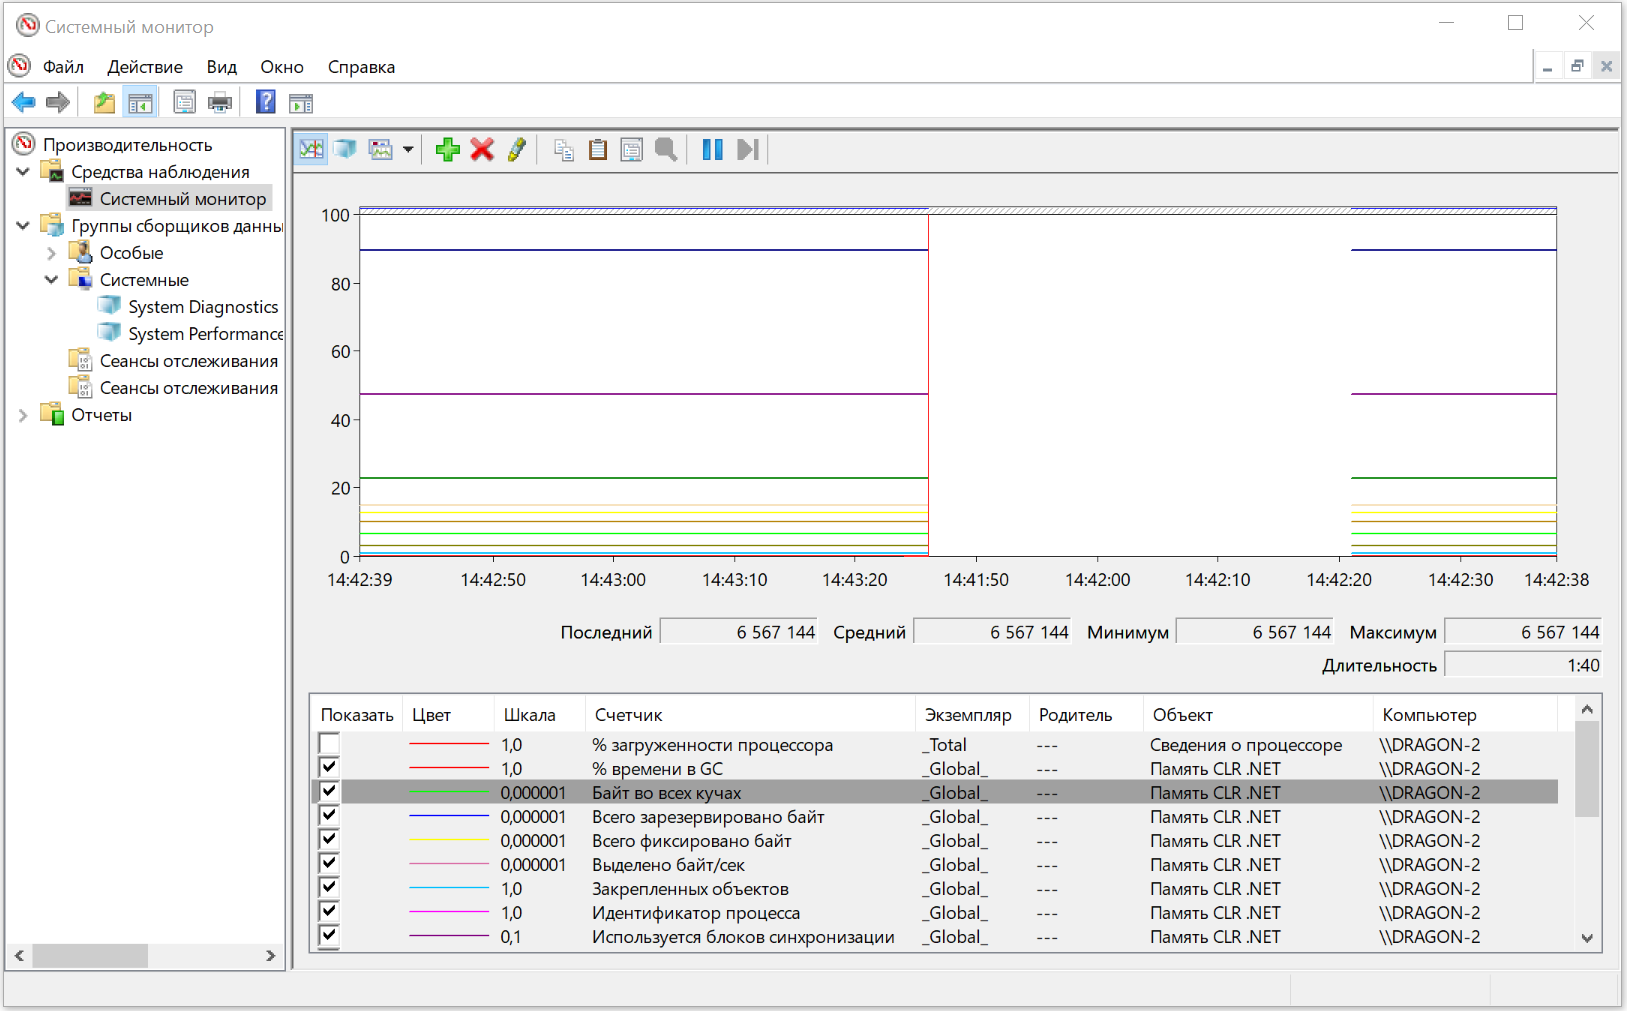
\includegraphics[width=0.7\textwidth]{perfMon.png}
		\end{center}
	\end{frame}

	\section{Финализаторы}

	\begin{frame}[fragile]
		\frametitle{Финализаторы}
		\begin{itemize}
			\item Если объекту требуется только память, то сборщик мусора всё сделает за нас, но бывает так, что требуются ещё системные ресурсы
			\begin{itemize}
				\item System.IO.FileStream, System.Threading.Mutex
			\end{itemize}
			\item Метод \textit{Finalize()}
			\item Финализатор (просто синтаксис для Finalize):
		\end{itemize}
		\begin{footnotesize}
			\begin{minted}{csharp}
internal sealed class SomeType {
    ~SomeType() {
        ...
    }
}
			\end{minted}
		\end{footnotesize}
		Не деструктор! Finalize вызывается, ``когда хочет''
	\end{frame}

	\begin{frame}
		\frametitle{Дьявол в деталях}
		\begin{itemize}
			\item Объекты с финализаторами всегда переживают сборку в своём поколении
			\begin{itemize}
				\item Сборщик мусора должен дать финализатору отработать
				\item Все поля объекта с финализатором тоже живут дольше, чем надо
			\end{itemize}
			\item Порядок вызова финализаторов не определён
			\begin{itemize}
				\item Из финализатора нельзя обращаться к объекту с финализатором
			\end{itemize}
			\item Финализаторы запускаются в отдельном потоке
			\begin{itemize}
				\item Нельзя рассчитывать на определённый поток
				\item Если Finalize повис, то всё, все финализируемые объекты будут жить вечно
				\item Если Finalize бросил исключение, то весь процесс аварийно завершается
			\end{itemize}
		\end{itemize}
	\end{frame}

	\begin{frame}[fragile]
		\frametitle{System.Runtime.InteropServices.SafeHandle}
		\begin{scriptsize}
			\begin{minted}{csharp}
public abstract class SafeHandle : CriticalFinalizerObject, IDisposable {
    protected IntPtr handle;

    protected SafeHandle(IntPtr invalidHandleValue, Boolean ownsHandle);
    protected void SetHandle(IntPtr handle);
    public void Dispose() { Dispose(true); }
    protected virtual void Dispose(Boolean disposing) {
        // The default implementation ignores the disposing argument.
        // If resource already released, return
        // If ownsHandle is false, return
        // Set flag indicating that this resource has been released
        // Call virtual ReleaseHandle method
        // Call GC.SuppressFinalize(this) to prevent Finalize from being called
        // If ReleaseHandle returned true, return
        // If we get here, fire ReleaseHandleFailed Managed Debugging Assistant (MDA)
    }
    ~SafeHandle() { Dispose(false); }
    protected abstract Boolean ReleaseHandle();
...
    public void DangerousAddRef(ref Boolean success) {...}
    public IntPtr DangerousGetHandle() {...}
    public void DangerousRelease() {...}
}
			\end{minted}
		\end{scriptsize}
	\end{frame}

	\begin{frame}[fragile]
		\frametitle{Пример, SafeFileHandle}
		\begin{scriptsize}
			\begin{minted}{csharp}
public sealed class SafeFileHandle : SafeHandleZeroOrMinusOneIsInvalid {
    public SafeFileHandle(IntPtr preexistingHandle, Boolean ownsHandle)
        : base(ownsHandle) {
        base.SetHandle(preexistingHandle);
    }

    protected override Boolean ReleaseHandle() {
        // Tell Windows that we want the native resource closed.
        return Win32Native.CloseHandle(base.handle);
    }
}
			\end{minted}
		\end{scriptsize}
	\end{frame}

	\section{IDisposable}

	\begin{frame}[fragile]
		\frametitle{IDisposable, так не работает}
		\begin{scriptsize}
			\begin{minted}{csharp}
public static class Program {
    public static void Main() {
        // Create the bytes to write to the temporary file.
         Byte[] bytesToWrite = new Byte[] { 1, 2, 3, 4, 5 };

        // Create the temporary file.
        FileStream fs = new FileStream("Temp.dat", FileMode.Create);

        // Write the bytes to the temporary file.
        fs.Write(bytesToWrite, 0, bytesToWrite.Length);

        // Delete the temporary file.
        File.Delete("Temp.dat"); // Throws an IOException
    }
}
			\end{minted}
		\end{scriptsize}
	\end{frame}

	\begin{frame}[fragile]
		\frametitle{IDisposable, так работает}
		\begin{scriptsize}
			\begin{minted}{csharp}
public static class Program {
    public static void Main() {
        // Create the bytes to write to the temporary file.
         Byte[] bytesToWrite = new Byte[] { 1, 2, 3, 4, 5 };

        // Create the temporary file.
        FileStream fs = new FileStream("Temp.dat", FileMode.Create);

        // Write the bytes to the temporary file.
        fs.Write(bytesToWrite, 0, bytesToWrite.Length);

        // Explicitly close the file when finished writing to it.
        fs.Dispose();

        // Delete the temporary file.
        File.Delete("Temp.dat"); // Throws an IOException
    }
}
			\end{minted}
		\end{scriptsize}
	\end{frame}

	\begin{frame}
		\frametitle{IDisposable, детали}
		\begin{itemize}
			\item Класс, реализующий IDisposable, должен уметь бросать System.ObjectDisposedException из всех своих методов и свойств
			\item Dispose не должен бросать исключение
			\begin{itemize}
				\item Если вызван несколько раз, то просто ничего не делать
			\end{itemize}
			\item Если вы явно вызываете Dispose из своего кода, вы, скорее всего, делаете что-то не так
			\item Dispose не обязан быть thread-safe
		\end{itemize}
	\end{frame}

	\begin{frame}[fragile]
		\frametitle{using}
		\begin{scriptsize}
			\begin{minted}{csharp}
public static class Program {
    public static void Main() {
        // Create the bytes to write to the temporary file.
        Byte[] bytesToWrite = new Byte[] { 1, 2, 3, 4, 5 };
        // Create the temporary file.
        using (FileStream fs = new FileStream("Temp.dat", FileMode.Create)) {
            // Write the bytes to the temporary file.
            fs.Write(bytesToWrite, 0, bytesToWrite.Length);
        }
        // Delete the temporary file.
        File.Delete("Temp.dat");
    }
}
			\end{minted}
		\end{scriptsize}
	\end{frame}

	\section{Финализация изнутри}

	\begin{frame}
		\frametitle{Финализация изнутри}
		\begin{itemize}
			\item Finalization list --- туда добавляются все объекты, переопределяющие Finalize(), в момент создания
			\item Freachable queue --- туда перекладываются объекты из Finalization list, которые должны умереть, в момент сборки мусора
		\end{itemize}
		\begin{center}
			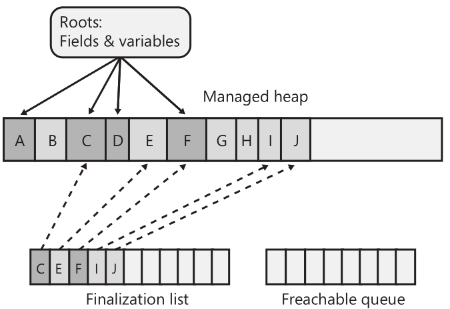
\includegraphics[width=0.4\textwidth]{finalizationList.png}
		\end{center}
	\end{frame}

	\begin{frame}
		\frametitle{Финализация изнутри (2)}
		\begin{itemize}
			\item Объекты из Freachable queue считаются сборщиком мусора root-ами и не умирают
			\item Финализаторы запускаются в отдельном потоке для каждого объекта из очереди
			\item Объекты выкидываются из очереди в процессе
		\end{itemize}
		\begin{center}
			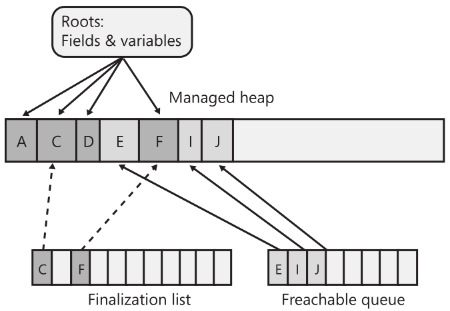
\includegraphics[width=0.4\textwidth]{freachableQueue.png}
		\end{center}
	\end{frame}

	\begin{frame}
		\frametitle{Финализация изнутри (3)}
		\begin{itemize}
			\item При сборке мусора в следующем поколении финализированные объекты собираются, потому что на них уже точно нет ссылок
		\end{itemize}
		\begin{center}
			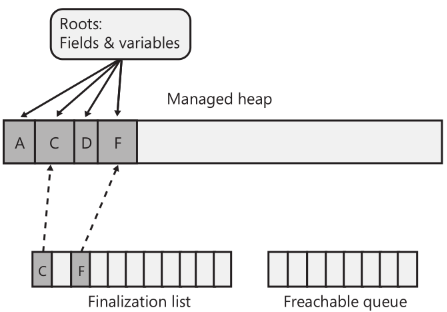
\includegraphics[width=0.4\textwidth]{finalizationDone.png}
		\end{center}
	\end{frame}

	\section{Ручное управление жизнью}

	\begin{frame}
		\frametitle{Ручное управление жизнью объекта}
		\begin{itemize}
			\item System.Runtime.InteropServices.GCHandle
			\begin{itemize}
				\item Value type, содержит указатель на запись в handle table
				\item Записи в handle table содержат объекты, но не все они считаются root-ами
			\end{itemize}
			\item GCHandleType:
			\begin{itemize}
				\item \textbf{Weak} --- позволяет узнать, что объект уже не нужен, но не факт, что финализатор отработал
				\item \textbf{WeakTrackResurrection} --- позволяет узнать, что объект уже не нужен и уже финализирован
				\item \textbf{Normal} --- просьба к GC держать объект в памяти, но можно двигать
				\item \textbf{Pinned} --- просьба к GC держать объект в памяти и не двигать
				\begin{itemize}
					\item Ключевое слово \textbf{fixed}
				\end{itemize}
			\end{itemize}
		\end{itemize}
	\end{frame}

	\begin{frame}[fragile]
		\frametitle{Пример, fixed}
		\begin{scriptsize}
			\begin{minted}{csharp}
unsafe public static void Go() {
    // Allocate a bunch of objects that immediately become garbage
    for (Int32 x = 0; x < 10000; x++) new Object();
    IntPtr originalMemoryAddress;
    Byte[] bytes = new Byte[1000]; // Allocate this array after the garbage objects

    // Get the address in memory of the Byte[]
    fixed (Byte* pbytes = bytes) { originalMemoryAddress = (IntPtr) pbytes; }

    // Force a collection; the garbage objects will go away & the Byte[] might be compacted
    GC.Collect();

    // Get the address in memory of the Byte[] now & compare it to the first address
    fixed (Byte* pbytes = bytes) {
        Console.WriteLine("The Byte[] did{0} move during the GC",
            (originalMemoryAddress == (IntPtr) pbytes) ? " not" : null);
    }
}
			\end{minted}
		\end{scriptsize}
	\end{frame}

	\begin{frame}[fragile]
		\frametitle{WeakReference}
		\begin{scriptsize}
			\begin{minted}{csharp}
public sealed class WeakReference<T> : ISerializable where T : class {
    public WeakReference(T target);
    public WeakReference(T target, Boolean trackResurrection);
    public void SetTarget(T target);
    public Boolean TryGetTarget(out T target);
}
			\end{minted}
		\end{scriptsize}
	\end{frame}

	\section{Заключение}

	\begin{frame}
		\frametitle{Заключение}
		Все примеры и картинки взяты из J. Richter, CLR via C\# (4th edition), Microsoft Press, 2012, 896pp
		\begin{center}
			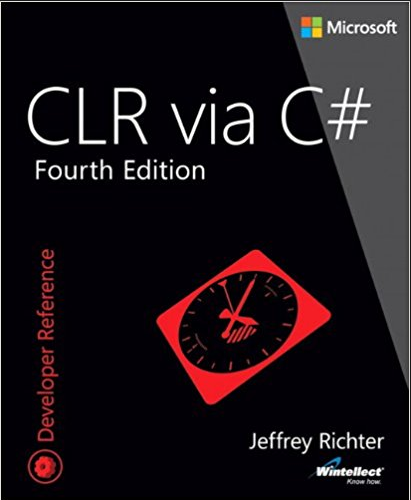
\includegraphics[width=0.35\textwidth]{richterCover.png}
		\end{center}
	\end{frame}

\end{document}
